\documentclass{report}
\usepackage{geometry}
\usepackage{paralist}
\usepackage{scalerel,amssymb}
\usepackage{tikz}
\usepackage{amsmath}
\usepackage{array}
\usepackage{nccmath}

\usepackage{fancyhdr}
\fancyhead[L]{\LARGE Applied Optimization \\
\Large Exercise 01}
\fancyhead[R]{13-123-922 \\
Elias Wipfli \\
13-933-262 \\
Lorenzo \textsl{Wipfli}  \\
16-124-836 \\
Marcel \textsc{Zauder}}
\renewcommand{\headrulewidth}{0.4pt}
\fancyfoot[C]{\thepage}
\renewcommand{\footrulewidth}{0.4pt}

\usepackage{hyperref}

\begin{document}
	\pagestyle{fancy}
	\hfill \\ \\
	
	\section*{1.1 Convex Sets}
	\subsection*{1.1.1 Example Sets}
	\begin{enumerate}[1.]
		\item span$\lbrace\left(^1_1\right) , \left(^{-0.5}_{-0.5}\right)\rbrace $ \\
		\begin{tabular}{m{4.5cm} m{7.5cm}}
			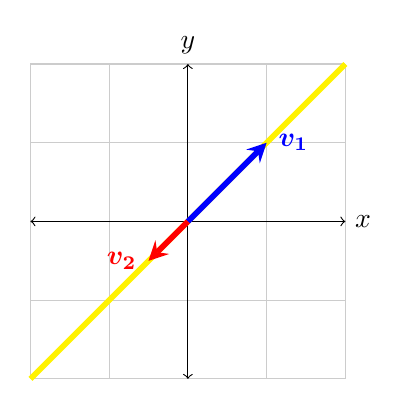
\begin{tikzpicture}
  				\draw[thin,gray!40] (-2,-2) grid (2,2);
  				\draw[<->] (-2,0)--(2,0) node[right]{$x$};
  				\draw[<->] (0,-2)--(0,2) node[above]{$y$};
  				\draw[line width=2pt, yellow](-2,-2)--(2,2);
  				\draw[line width=2pt,blue,-stealth](0,0)--(1,1) node[anchor=west]{$\boldsymbol{v_1}$};
 				\draw[line width=2pt,red,-stealth](0,0)--(-0.5,-0.5) node[anchor=east]{$\boldsymbol{v_2}$};
			\end{tikzpicture}
			&
			\begin{tabular}{c}
				span$\lbrace\left(^1_1\right) , \left(^{-0.5}_{-0.5}\right)\rbrace $ is a line through the origin \\ 
			because the vectors are linear dependent.
			\end{tabular}
		\end{tabular}
		\item span$\lbrace\left(^1_1\right) , \left(^{\ 0.5}_{-0.5}\right)\rbrace $ \\
		\begin{tabular}{m{4.5cm} m{7.5cm}}
			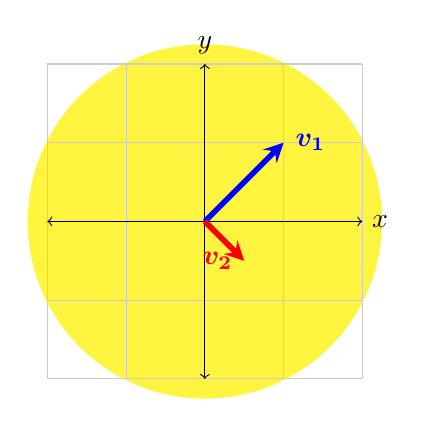
\begin{tikzpicture}
				\pgfdeclarelayer{bg}
				\pgfsetlayers{bg,main}
				\draw[thin,gray!40] (-2,-2) grid (2,2);
  				\draw[<->] (-2,0)--(2,0) node[right]{$x$};
  				\draw[<->] (0,-2)--(0,2) node[above]{$y$};
  				\draw[line width=2pt,blue,-stealth](0,0)--(1,1) node[anchor=west]{$\boldsymbol{v_1}$};
 				\draw[line width=2pt,red,-stealth](0,0)--(0.5,-0.5) node[anchor=east]{$\boldsymbol{v_2}$};
 				\begin{pgfonlayer}{bg} 
        			\node[circle, fill=yellow!75, minimum height=4.5cm] (circle-bg) {};
    			\end{pgfonlayer}
 				 
			\end{tikzpicture}
			&
			\begin{tabular}{c}
				span$\lbrace\left(^1_1\right) , \left(^{\ 0.5}_{-0.5}\right)\rbrace $ is the whole $\mathbb{R}^2$ plane \\ 
			because the vectors are linear independent.
			\end{tabular}
		\end{tabular}
		\item aff$\lbrace\left(^1_0\right) , \left(^{\ 1}_{-1}\right)\rbrace $ \\
		\begin{tabular}{m{4.5cm} m{7.5cm}}
			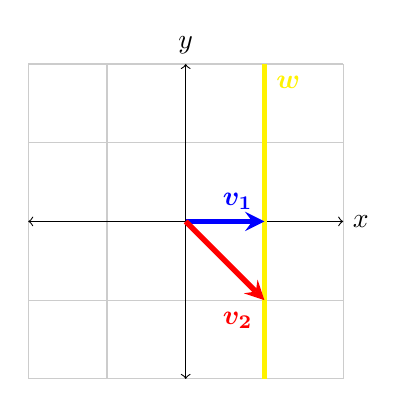
\begin{tikzpicture}
  				\draw[thin,gray!40] (-2,-2) grid (2,2);
  				\draw[<->] (-2,0)--(2,0) node[right]{$x$};
  				\draw[<->] (0,-2)--(0,2) node[above]{$y$};
  				\draw[line width=2pt, yellow](1,-2)--(1,2) node[anchor=north west]{$\boldsymbol{w}$};
  				\draw[line width=2pt,blue,-stealth](0,0)--(1,0) node[anchor=south east]{$\boldsymbol{v_1}$};
 				\draw[line width=2pt,red,-stealth](0,0)--(1,-1) node[anchor=north east]{$\boldsymbol{v_2}$};
			\end{tikzpicture}
			&
			\begin{tabular}{c}
				aff$\lbrace\left(^1_0\right) , \left(^{\ 1}_{-1}\right)\rbrace $ creates a line w with: \\
				 $w = v_1 + \beta (v_2 - v_1) = \left(^1_0\right) + \beta \left(^{\ 0}_{-1}\right)$ \\
				 which is a line parallel to the y-axis.
			\end{tabular}
		\end{tabular}
		\item conv$\lbrace\left(^1_0\right) , \left(^2_1\right) , \left(^{\ 3}_{-2}\right), \left(^{-1}_{\ 0}\right) , \left(^{-2}_{\ 1}\right) , \left(^{-2}_{-2}\right)\rbrace $ \\
		\begin{tabular}{m{7cm} m{7.5cm}}
			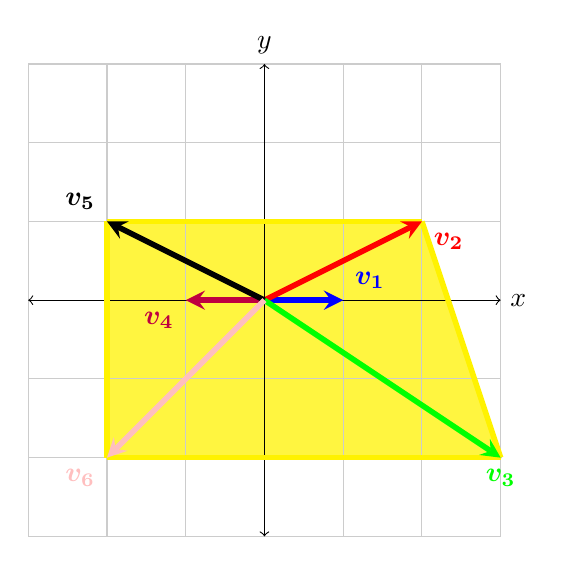
\begin{tikzpicture}
				\draw[fill=yellow!75]  (2,1) -- (3,-2) -- (-2,-2) -- (-2,1) -- cycle;
  				\draw[thin,gray!40] (-3,-3) grid (3,3);
  				\draw[<->] (-3,0)--(3,0) node[right]{$x$};
  				\draw[<->] (0,-3)--(0,3) node[above]{$y$};
  				\draw[line width=2pt, yellow](2,1)--(3,-2);
  				\draw[line width=2pt, yellow](2,1)--(-2,1);
  				\draw[line width=2pt, yellow](-2,1)--(-2,-2);
  				\draw[line width=2pt, yellow](-2,-2)--(3,-2);
  				\draw[line width=2pt,blue,-stealth](0,0)--(1,0) node[anchor=south west]{$\boldsymbol{v_1}$};
 				\draw[line width=2pt,red,-stealth](0,0)--(2,1) node[anchor=north west]{$\boldsymbol{v_2}$};
 				\draw[line width=2pt,green,-stealth](0,0)--(3,-2) node[anchor=north]{$\boldsymbol{v_3}$};
 				\draw[line width=2pt,purple,-stealth](0,0)--(-1,0) node[anchor=north east]{$\boldsymbol{v_4}$};
 				\draw[line width=2pt,black,-stealth](0,0)--(-2,1) node[anchor=south east]{$\boldsymbol{v_5}$};
 				\draw[line width=2pt,pink,-stealth](0,0)--(-2,-2) node[anchor=north east]{$\boldsymbol{v_6}$};
			\end{tikzpicture}
			&
			\begin{tabular}{c}
				conv$\lbrace\left(^1_0\right) , \left(^2_1\right) , \left(^{\ 3}_{-2}\right), \left(^{-1}_{\ 0}\right) , \left(^{-2}_{\ 1}\right) , \left(^{-2}_{-2}\right)\rbrace $ \\
				creates a quadrilateral with the vertices \\
				$v_2,v_3,v_5$ and $v_6$. $v_1$ and $v_4$ are inside the \\
				shape so there wouldn't be a difference in \\
				the shape if they were missing.
			\end{tabular}
		\end{tabular}
	\end{enumerate}
	\hfill \\
	
	\subsection*{1.1.2 Convexity}
	$C \in \mathbb{R}^n$, $x_1, x_2, ... , x_k \in C$, $\theta_1, ... , \theta_k \in \mathbb{R}$, $\theta_i \geq 0$, $\theta_1 + ... + \theta_k =1$ \\
	\textbf{\textsc{Show:}} $\theta_1 x_1 + ... + \theta_k x_k \in C$
	\begin{align*}
		\pmb{\underline{k=2:}} \ \ \ \ \ \ \ \ & \theta_1 x_1 + \theta_2 x_2 \stackrel{?}{\in} C \\
		& \theta_1 + \theta_2 = 1 \Rightarrow \theta_2 = 1 - \theta_1 \\
		& \Rightarrow \theta_1 x_1 + (1-\theta_1) x_2 \\
		& = \theta_1 x_1 + x_2 - theta_1 x_2 \\
		& = \theta_1 (x_1-x_2) + x_2 \in C 
	\end{align*}
	\begin{align*}
		\pmb{\underline{k > 2:}} \ \ \ \ \ \ \ \ & u = \sum^{k-1}_{i=1} \theta_i = 1 - \theta_k \\
		& \textit{if } u=0, \textit{ then } \sum^k_{i=1} \theta_i x_i = x_k \in C \\
		& \textit{else let } a_i = \frac{\theta_i}{u}, w := \sum^{k-1}_{i=1} a_i x_i \in C, \textit{ because } \sum^{k-1}_{i=1} a_i = 1 \textit{ and all } a_i \geq 0 \\
		& \textit{Then } \sum^k_{i=1} \theta_i x_i = x_k + u \cdot (w-x_k) \textit{ is a point in the line segment } x_k \textit{ to } w, \textit{ hence in C.} \\ 
		& \square
	\end{align*}
	
	\subsection*{1.1.3 Linear Equations}
	Show that the solution set of linear equations $\{x \mid Ax=b\} \in C$ with $x \in \mathbb{R}^n$, $A \in \mathbb{R}^{m \times n}$ and $b \in \mathbb{R}^m$ is an affine set.
	\begin{align*}
		& \textit{If } Ax \neq b, \textit{ then } \{x \mid Ax = b\} \textit{ is empty and empty sets are affine.} \\
		& \textit{If } Ax = b: \\
		& \textit{suppose } x_1, x_2 \in C, \  Ax_1 = b, \  Ax_2 = b \\
		& \textit{Then for any } \theta, \textit{ we have:} \\
		& A(\theta x_1 + (1-\theta)x_2) \\ 
		& = \theta Ax_1 + (1-\theta) Ax_2 \\
		& = \theta b + (1-\theta)b \\
		& = b \\
		& \textit{which shows that the affine combination } \theta x_1 + (1-\theta)x_2 \textit{ is also in C.}
	\end{align*}
	
	\subsection*{1.1.4 Linear Inequations}
	\begin{enumerate}[1.]
		\item Proof of a convex set
		\begin{enumerate}[]
			\item Show that the solution set of linear inequalities $\{x \mid Ax \preceq b, Cx = d\}$ with $x\in \mathbb{R}^n, \ A \in \mathbb{R}^{m \times n}, \ b \in \mathbb{R}^m, \ C \in \mathbb{R}^{k\times n }, \ d \in \mathbb{R}^k$ is a convex set.
			\item Assumption:
			\[
				x_1, x_2 \in \{x \mid Ax \preceq b, Cx =d\} $$ $$
				Ax_1 \preceq b, \ x_1 \geq 0, \ Ax_2 \preceq b, \ x_2 \geq 0 \textit{ with } \lambda \in [0,1]:
			\]
			\begin{align*}
				\lambda Ax_1 \ & \preceq \ \lambda b \\
				(1-\lambda)Ax_2 \ & \preceq \ (1-\lambda) b \\
				\Rightarrow A(\lambda x_1 + (1-\lambda ) x_2) \ & \preceq \ b \\
				\Rightarrow \ \ \ \ \ \lambda x_1 + (1-\lambda ) x_2 \ & \succeq \ 0
			\end{align*}
			\item Vector a and scalar b, suppose x and y satisfy:
			\[
				a^{\top}x \geq b \textit{ and } a^{\top}y \geq b
			\]
			, therefore belong to the same halfspace.
			\[
				\textit{For a }\lambda \in [0,1]: \ \ \ \ \ \ \ \ \ \ \ \ \ \ \ \ a^{\top}(\lambda x + (1-\lambda ) y) \geq \lambda b + (1-\lambda ) b = b
			\]
			, which proves that $\lambda x + (1-\lambda ) y$ also belongs to the halfspace. \\
			Therefore a halfspace is convex and since a polyhedron is the intersecion of a finite number of halfspaces, it is also convex. $\square$
		\end{enumerate}
		\item Is it an affine set?
		\begin{enumerate}[]
			\item No, it is not halfspaces themself are not affine and by intersecting them you cannot get an affine set.
		\end{enumerate}
	\end{enumerate}
	
	\subsection*{1.1.5 Voronoi description of halfspaces}
	a,b distinct points in $\mathbb{R}^n$, with:
	\[
	\{x\mid \| x-a \|_2 \leq \| x-b \|_2\}
	\]
	Show that this is a halfspace: \\
	A norm is alway nonnegative, so $\| x-a \|_2 \leq \| x-b \|_2$ holds if and only if $\| x-a \|^2_2 \leq \| x-b \|^2_2$, so:
	\begin{align*}
		\| x-a \|^2_2 \ & \leq \ \| x-b \|^2_2 \\
		\Leftrightarrow \ \ \ (x-a)^{\top}(x-a) \ & \leq \ (x-b)^{\top}(x-b) \\
		\Leftrightarrow \ \ \ x^{\top}x - 2a^{\top}x + a^{\top}a \ & \leq \ x^{\top}x - 2b^{\top}x + b^{\top}b \\
		\Leftrightarrow \ \ \ 2(b-a)^{\top}x \ & \leq \ b^{\top}b - a^{\top}a	
	\end{align*}
	So c = 2(b-a) and d = $b^{\top}b - a^{\top}a$, points that are equidistant to A and B are given by a hyperplane with the normal $\frac{b-a}{\mid b-a \mid}$. \\
	\textbf{\textsc{\underline{Picture:}}} \\
	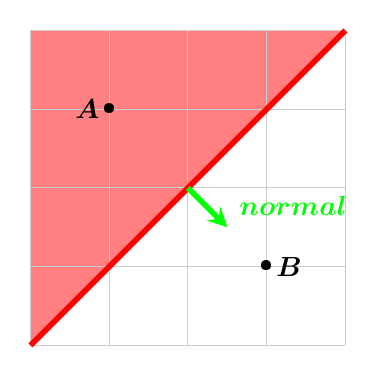
\begin{tikzpicture}
		\draw[fill=red!50] (-2,-2) -- (-2,2) -- (2,2);
  		\draw[thin,gray!40] (-2,-2) grid (2,2);
  		\draw[line width=2pt, red](-2,-2)--(2,2);
  		\foreach \Point in {(-1,1) , (1,-1)}{
  			\node at \Point {\textbullet};
  		}
  		\draw (-1,1) node[anchor=east]{$\boldsymbol{A}$};
  		\draw (1,-1) node[anchor=west]{$\boldsymbol{B}$};
  		\draw[line width=2pt,green,-stealth](0,0)--(0.5, -0.5) node[anchor=south west]{$\boldsymbol{normal}$};
	\end{tikzpicture}
	
	\section*{1.2 Convex Functions}
	\subsection*{1.2.1 Convexity Test}
	The function isConvex() was implemented straight forward with the given convexity theorem.
	For the first function that is evaluated we get quite quickly the points that are not concave.\\ For the second function:
					\[
				  f(\theta x+(1-\theta)y)=1/2((\theta x+(1-\theta)y)^{\top}A(\theta x+(1-\theta)y)+ b^{\top}(\theta x+(1-\theta)y) + c = $$ $$
				  1/2(\theta x^{\top}A\theta x + (1-\theta)y^{\top}A(1-\theta)y) + b^{\top}\theta x + b^{\top}(1-\theta)y+ c =$$ $$ 
				  1/2\ \theta^{2}(x^{\top}Ax) + 1/2\ (1-\theta)^{2}(y^{\top}Ay)+ b^{\top}\theta x + b^{\top}(1-\theta)y+ c
			\]
			And:
			\[
			\theta f(x)+(1-\theta)f(y)= \theta (1/2 x^{\top}Ax+b^{\top}x+c) + (1-\theta)(1/2 y^{\top}Ay+b^{\top}y+c)= $$ $$
			 1/2 \ \theta \  (x^{\top}Ax) + 1/2 \ (1-\theta) \  (y^{\top}Ay) + b^{\top}\theta x + b^{\top}(1-\theta)y + \theta c + (1-\theta) c = $$ $$
			 1/2 \ \theta \  (x^{\top}Ax) + 1/2 \ (1-\theta) \  (y^{\top}Ay) + b^{\top}\theta x + b^{\top}(1-\theta)y + c			
			\]
			Because we know that: $$0 \leq \theta \leq 1$$
			We can see that:
			\[
			1/2 \ \theta^{2} \  (x^{\top}Ax)  \leq  1/2 \ \theta \  (x^{\top}Ax)
			\]
						\[
			1/2 \ (1-\theta)^{2} \ (y^{\top}Ay)  \leq 1/2 \ (1-\theta) \  (y^{\top}Ay)
			\]
The rest is the same in both formulas so:
			\[
f(\theta x+(1-\theta)y) \leq \theta f(x)+(1-\theta)f(y) \ \square
			\]
			So the second function is convex.
	\section*{1.3 Convex Illumination Problem}
	@ Holy moly, imma out of here!
	
\end{document}